\documentclass{beamer}

\usepackage{mystyle} % import all packages listed in mystyle.sty

\usetheme{Rochester}
\usecolortheme{crane}

\beamertemplatenavigationsymbolsempty

\title{Introduction to \LaTeX{}}
\subtitle{A Quick Crash Course}
\author{Amin Mesbah}
\date{15 April, 2016}

\begin{document}

    \frame{\titlepage}
    
    \frame{
        \frametitle{What is \LaTeX{}?}
        \begin{itemize}
            \item A document typesetting markup language
            \item A tool that can save you a lot of time
            \item Commonly used to write research papers, but useful for many other things too (resumes, calendars, posters, books, letters, notes, this slideshow...)
        \end{itemize}
    }

    \frame{
        \frametitle{Setup}
        \begin{itemize}
            \item Windows: \href{http://miktex.org/}{\underline{MiKTeX}} 
            \item Mac: \href{https://tug.org/mactex/}{\underline{MacTeX}}
            \item Linux: \code{apt-get install texlive}
            \item Online:
            \begin{itemize}
                \item \href{https://www.overleaf.com/}{\underline{Overleaf}}
                \item \href{https://www.sharelatex.com/}{\underline{ShareLatex}}
            \end{itemize}
        \end{itemize}
    }

    \frame{
        \frametitle{Using Overleaf}
        Go to overleaf.com and click "Create a New Paper". \\
        Then click "Source"
    }

    \frame[plain]{
        \begin{center}
        \hspace*{-1.2cm}
        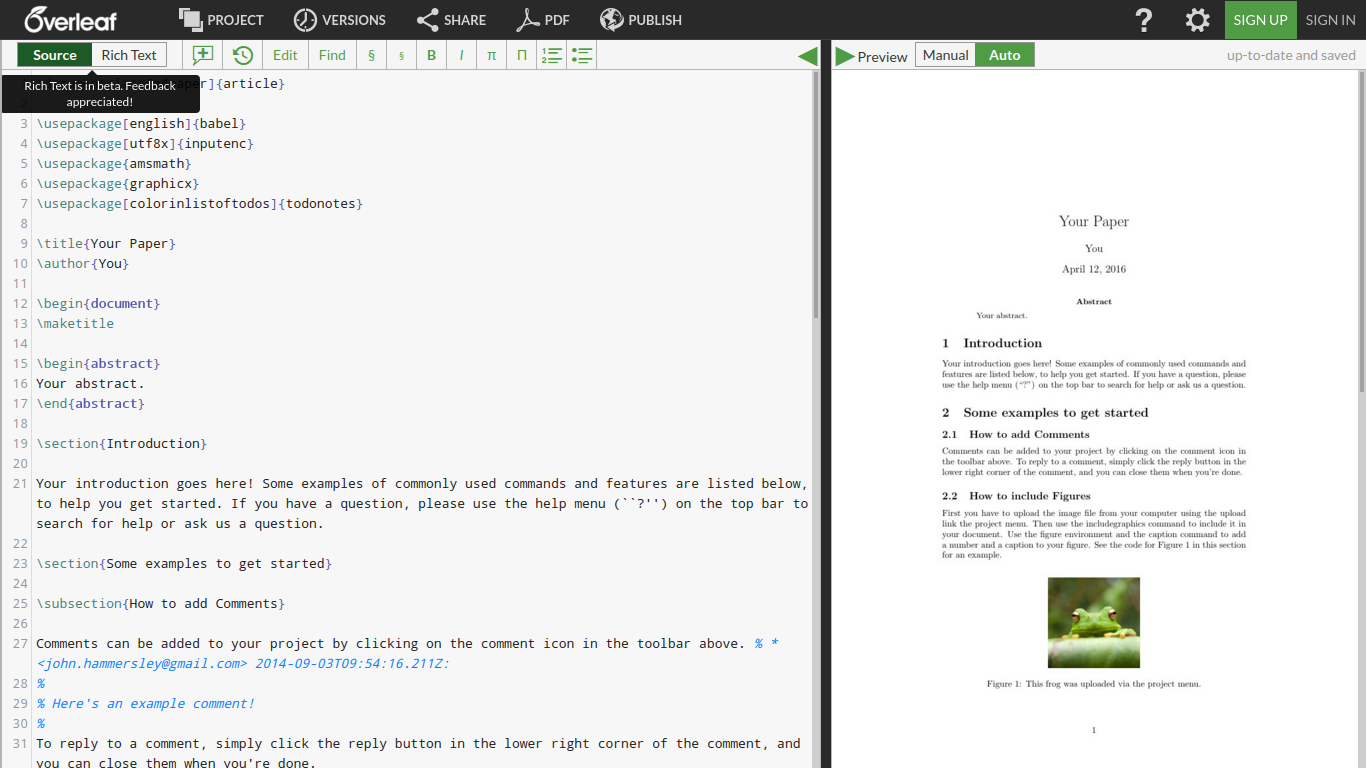
\includegraphics[scale=0.3]{img/overleafsource}
        \end{center}
    }

    \frame{
        \frametitle{"Hello, World!"}
        \framesubtitle{Making our first \LaTeX{} document}
        A \LaTeX{} document has two main parts (called environments):
        \begin{itemize}
            \item Preamble Environment
                \begin{itemize}
                \item Set up the rules for how your document will look
                \end{itemize}
            \item Document Environment
                \begin{itemize}
                \item The place where you write your document
                \end{itemize}
        \end{itemize}
    }

    \frame{
        \frametitle{The Code for \code{helloworld.tex}}
        \framesubtitle{Making our first \LaTeX{} document}
        \lstinputlisting[language=TeX]{"./code-snippets/hello-world.tex"}
    }

    \frame{
        \frametitle{Let's add a Title!}
        \framesubtitle{Making our first \LaTeX{} document}
        \lstinputlisting[language=TeX]{"./code-snippets/hello-world-title.tex"}
    }

    \frame[shrink]{
        \frametitle{Adding Graphics from Mathematica}
        \framesubtitle{Making our first \LaTeX{} document}

        First add the \code{graphicx} package in your documents preamble:
        \lstinputlisting[language=TeX, firstline=4, lastline=4]{"./code-snippets/hello-world-image.tex"}

        Then add the following code to your document's body:
        \lstinputlisting[language=TeX, firstline=15, lastline=16]{"./code-snippets/hello-world-image.tex"}
    }

    \frame[shrink]{
        \frametitle{Adding a table}
        \framesubtitle{Making our first \LaTeX{} document}
        \lstinputlisting[language=TeX, firstline=12, lastline=27]{"./code-snippets/hello-world-table.tex"}
    }

    \frame{
        \frametitle{The Math Environment}
        \begin{itemize}
            \item \LaTeX{} was originally designed to make it easy to write nice looking mathematical notation.
            \item If you want to write math, use the \code{amsmath} package.
            \item Since math formulas need to look different than normal text, they go in their own special math environment.
        \end{itemize}
    }

    \frame[shrink]{
        \frametitle{Adding Math}
        \framesubtitle{Making our first \LaTeX{} document}
        First add the \code{amsmath} package in your document's preamble:
        \lstinputlisting[language=TeX, firstline=3, lastline=3]{"./code-snippets/hello-world-math.tex"}

        Then add the following code to your document's body:
        \lstinputlisting[language=TeX, firstline=14, lastline=27, breaklines=true]{"./code-snippets/hello-world-math.tex"}
    }

    \frame{
        \frametitle{A More Advanced Example}
        Start a new project and load \code{basic-example.tex} from the examples folder \\

        Look at the code. There are some things we've already covered, and some other things we haven't.
    }

\begin{comment}
    \frame{
        \frametitle{LaTeX for Lab Reports}
    }

\end{comment}

    \frame{
        \frametitle{Resources}
        Learning \LaTeX takes time. These resources will help:
        \begin{itemize}
            \item \href{http://latextemplates.com/}{\underline{Templates!}}
            \item \href{http://bamos.github.io/latex-templates/}{\underline{More Templates!}}
            \item \href{https://overleaf.com/latex/templates}{\underline{Even More Templates!}}
            \item \href{https://en.wikibooks.org/wiki/LaTeX}{\underline{\LaTeX{} Wikibook}}
            \item \href{https://learnxinyminutes.com/docs/latex/}{\underline{A quick introduction}}
            \item \href{http://mecmath.net/latex-tutorial.pdf}{\underline{Mini Tutorial}}
            \item \href{http://tex.stackexchange.com}{\underline{Question and Answer Community}}
        \end{itemize}

        Google is your friend: \href{https://www.google.com/search?q=latex+integral+symbol}{\underline{How do I make an integral symbol in latex?}}
}

\end{document}
